\chapter{PROPOSAL} \label{ch:procedure}

\section{Functional Requirements:}

\subsection{Multi-Tenant Architecture and Secure Vendor Management}
The system shall provide a multi-tenant architecture where entrepreneurs can register, pay for subscriptions, and operate independent digital storefronts. To ensure strict privacy and prevent data leakage between competing vendors, the system must utilize a "Database-per-Tenant" design for data isolation and enforce proper verification for vendor access.



\subsection{Comprehensive Store Operations and Inventory Management}
The system shall equip vendors with a centralized dashboard to fully control their storefront's operations and interface. This includes real-time inventory synchronization, the creation of promotional offers and customizable discounts, analytics tracking, and the ability to customize the store's visual themes and layout.


\subsection{Integrated Checkout, Payment, and Order Fulfillment}
The system shall facilitate a seamless purchasing workflow for end-customers by supporting multiple payment methods, including secure online gateways (bKash, Nagad, Visa, MasterCard) and Cash on Delivery (COD). Additionally, the system must integrate with third-party logistics APIs (like Pathao or RedX) to provide automated, real-time product delivery tracking for both customers and vendors.


\section{Non-Functional Requirements}

\subsection{Data Isolation \& Security (Confidentiality)}
Metric: Since we are using a multi-tenant "Database-per-Tenant" design, the system must ensure 100\% data isolation. No cross-tenant query should be possible.

\subsection{Scalability \& Performance}
Metric: The Analytical Board and Inventory Management systems must handle concurrent updates. The system should maintain a response time of < 2 seconds for dashboard loading, even when 500+ vendors are accessing their respective databases simultaneously.

\subsection{High Availability \& Reliability}
Metric: Given that this is a subscription-based "Independent Storefront" model, the system must guarantee 99.9\% uptime. If the Payment Gateway or the Database-per-Tenant service fails, it must have a failover mechanism so vendors don't lose sales during peak promotional hours.

\section{User Stories}

\subsection{User Story for Multi-Tenant Architecture and Secure Vendor Management}

As an \textbf{entrepreneur (vendor)}, I want to register my business and subscribe to the platform to create my own digital storefront, so that I can manage products, customers, and orders online. The system should ensure that each vendor’s data is stored in an isolated database, preventing access by other vendors. Additionally, secure authentication and verification mechanisms must be implemented to protect vendor accounts and business information.

\subsection{User Story for Comprehensive Store Operations and Inventory Management}

As a \textbf{vendor}, I want to manage my store operations through a centralized dashboard, so that I can easily control inventory, create promotional offers, track sales analytics, and customize the visual appearance of my storefront. The system should provide real-time inventory updates and operational tools, enabling vendors to efficiently manage their online business from a single platform.

\subsection{User Story for Integrated Checkout, Payment, and Order Fulfillment}

As a \textbf{customer}, I want to complete purchases using multiple payment options such as online payment or Cash on Delivery, so that I can choose the most convenient payment method. The system should also integrate with third-party delivery services to provide real-time order tracking, allowing both customers and vendors to monitor the shipment status easily.

\section{Use Case Diagram}

\begin{figure}[H]
    \centering
    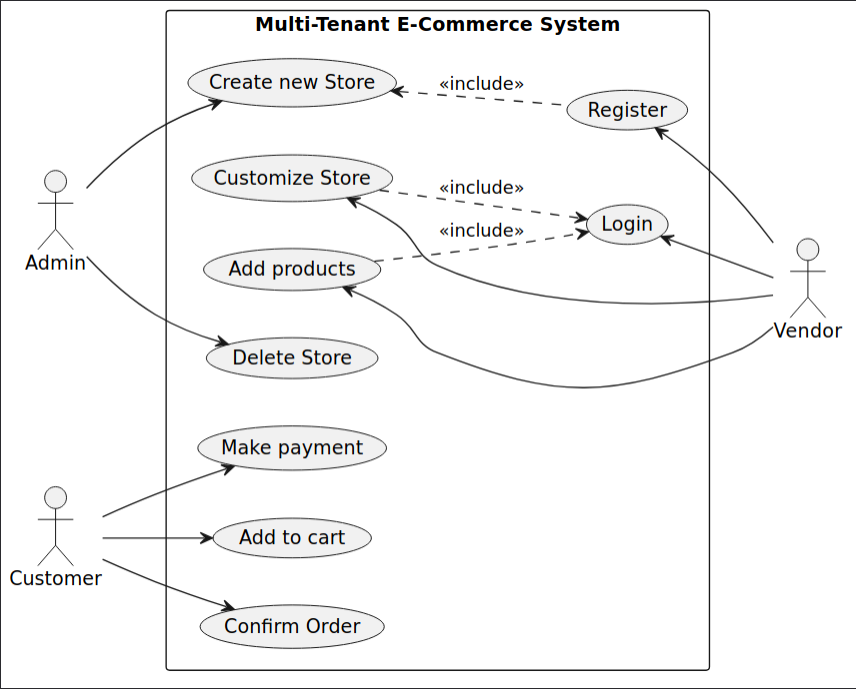
\includegraphics[width=1\linewidth]{figures/UseCaseDiagaram.png}
    \caption{Use Case Diagram for Multi-Tenants E-Commerce System}
    \label{fig:placeholder}
\end{figure}

\section{Use Case Specifications}

\subsection{Vendor Registration and Store Creation}

\textbf{Use Case Name:} Vendor Registration and Store Creation

\textbf{Actor}: Vendor (Entrepreneur)

\textbf{Description:} Allows entrepreneurs to register their business, subscribe
to the platform, and create an independent digital storefront with
isolated data storage.

\textbf{Preconditions:} Vendor has valid business and contact information. -
Vendor has internet access.

\begin{comment}
\textbf{Main Flow:} 1. Vendor enters business registration details. 2. Vendor
selects a subscription plan. 3. Vendor completes account verification
(email/OTP). 4. Platform creates a digital storefront with isolated
database.
\end{comment}

\textbf{Postconditions:} Vendor account is created and verified. - Independent
storefront is activated with isolated data storage.

\subsection{Store Operations and Inventory Management}

\textbf{Use Case Name:} Store Operations and Inventory Management

\textbf{Actor:} Vendor

\textbf{Description:} Allows vendors to manage store operations through a
centralized dashboard including product management, inventory updates,
promotions, analytics, and storefront customization.

\textbf{Preconditions:} Vendor account exists. - Vendor is logged into the
platform.

\begin{comment}    
\textbf{Main Flow:} 1. Vendor accesses the dashboard. 2. Vendor adds or updates
product listings and inventory. 3. Vendor creates promotional offers or
discounts. 4. Vendor views sales analytics and customizes storefront
appearance.
\end{comment}

\textbf{Postconditions:} Store products, inventory, and promotions are
updated. - Storefront configuration changes are applied.

\subsection{Checkout, Payment, and Order Tracking}

\textbf{Use Case Name:} Product Purchase and Order Fulfillment

\textbf{Actor:} Customer

\textbf{Description:} Allows customers to purchase products using multiple payment
methods and track order delivery through integrated logistics services.

\textbf{Preconditions:} Customer selects products. - Products are available in
stock.

\begin{comment} 
\textbf{Main Flow:} 1. Customer adds products to the shopping cart. 2. Customer
proceeds to checkout and enters delivery details. 3. Customer selects
payment method (online payment or Cash on Delivery). 4. Order is
confirmed and sent for delivery.
\end{comment}

\textbf{Postconditions:} Order is recorded in the system. - Customer and vendor
can track the delivery status.
